\documentclass[11pt,titlepage,twoside]{article}
\usepackage{geometry}                % See geometry.pdf to learn the layout options. There are lots.
\geometry{letterpaper}                   % ... or a4paper or a5paper or ... 
%\geometry{landscape}                % Activate for for rotated page geometry
%\usepackage[parfill]{parskip}    % Activate to begin paragraphs with an empty line rather than an indent
\usepackage{graphicx}
\usepackage{amssymb}
\usepackage{epstopdf}
\usepackage{url}
\usepackage{hyperref}
\usepackage{fancyhdr}
%\DeclareGraphicsRule{.tif}{png}{.png}{`convert #1 `dirname #1`/`basename #1 .tif`.png}

\def\ProgramVersionNoSpace{{VERSION}}
\def\ProgramVersion{{\ProgramVersionNoSpace \space}}
\def\ImagePath{{images}}

\title{PSF Estimator \ProgramVersion User Guide}
\author{Cory Quammen}
%\date{}                                           % Activate to display a given date or no date

\usepackage{fancyhdr}
\setlength{\headheight}{15pt}
 
\pagestyle{fancy}
 
\fancyhf{}
\fancyhead[LE,RO]{\thepage}
\fancyhead[RE]{\textit{PSF Estimator \ProgramVersion User Guide}}
\fancyhead[LO]{\textit{\nouppercase{\leftmark}}}
 
\fancypagestyle{plain}{ %
\fancyhf{} % remove everything
\renewcommand{\headrulewidth}{0pt} % remove lines as well
\renewcommand{\footrulewidth}{0pt}}

\begin{document}
\maketitle
\tableofcontents
\vfill

\pagebreak

\section{Introduction}

PSF Estimator is a program for computing a noise-free estimate of a point-spread function (PSF) of widefield and confocal microscopes. It works by fitting an analytical model of the PSF to an image of a sub-diffraction-limit-sized fluorescent bead. The fitting is a a maximum likelihood estimate that assumes noise is either Gaussian distributed;.

\subsection{System Requirements}

PSF Estimator \ProgramVersion requires Windows XP, Windows 7, or Macintosh OS X 10.5 or higher running on an Intel processor. A recent graphics card is recommended.

Your system should have at least 150 MB of hard drive space free to install the program. At least 512 MB of RAM is required, but 2 GB is recommended.

\subsection{Acknowledgements}

PSF Estimator \ProgramVersion is developed and maintained by the \href{http://www.cismm.org}{Center for Computer Integrated Systems for Microscopy and Manipulation}, a \href{http://www.nibib.nih.gov/}{National Institute of Biomedical Imaging and Bioengineering Resource}, award number P41-EB002025.

\section{Installation}

Installation of PSF Estimator \ProgramVersion is similar to installation of any other program.

\subsection{Getting the software}

To obtain the latest installer for PSF Estimator \ProgramVersionNoSpace, visit \url{http://www.cismm.org/downloads}. Please choose either the Mac or Windows version of the program, whichever is suitable for your system.

Source code for the program is also available there in the form of a Git repository, enabling you full access to the algorithms used to generate the images and providing the opportunity to submit bug fixes back to the project. 

\subsection{Windows installation}

Double-click the setup program named \textbf{PSFEstimator-\ProgramVersionNoSpace-win32.exe}. On the first screen, click \emph{Next}. Please read the program license. If you agree to the terms of the license, click \emph{I Agree}. On the next screen, choose where you want to install the program. The default directory is the most-used option. Click \emph{Next}. You may optionally choose a different location in the Start Menu. By default, it will be placed in the CISMM folder. Click \emph{Install}.

\subsection{Mac installation}

Double-click the Macintosh disk image named \textbf{PSFEstimator-\ProgramVersionNoSpace-darwin.dmg}. An installer program will launch and ask you to agree to the terms of the license. If you agree, a disk image named \textbf{PSFEstimator-\ProgramVersionNoSpace-Darwin} will appear on your desktop and a new Finder window will open.

To install the program in your \emph{Applications} directory on your computer's hard drive, drag the PSF Estimator \ProgramVersion application to either the \emph{Applications} alias in the Finder window that just appeared or drag it directly to your \emph{Applications} directory.

\subsection{Running the program}

\subsubsection{Windows}

You can launch the PSF Estimator program from the Start menu. If you chose the default installation location and menu folder, select \emph{Start} $\rightarrow$ \emph{All Programs} $\rightarrow$ \emph{PSF Estimator \ProgramVersionNoSpace} $\rightarrow$ \emph{PSF Estimator \ProgramVersionNoSpace}.

\subsubsection{Macintosh}

If you installed the application in the \emph{Applications} directory on your hard drive, double-click the program \emph{PSF Estimator \ProgramVersionNoSpace}.

\subsection{Where to get help}

If you have trouble installing or running the program or have questions about its usage, please please contact  \href{mailto:cquammen@cs.unc.edu}{Cory Quammen $\langle$cquammen@cs.unc.edu$\rangle$}. Unfortunately, no guarantee of support can be provided, but we will do our best to help you solve your problem.

\section{Getting to know PSF Estimator}

This section gives a tour of the many features in PSF Estimator.

\subsection{Program Window}

\begin{figure}[h]
  \centering
  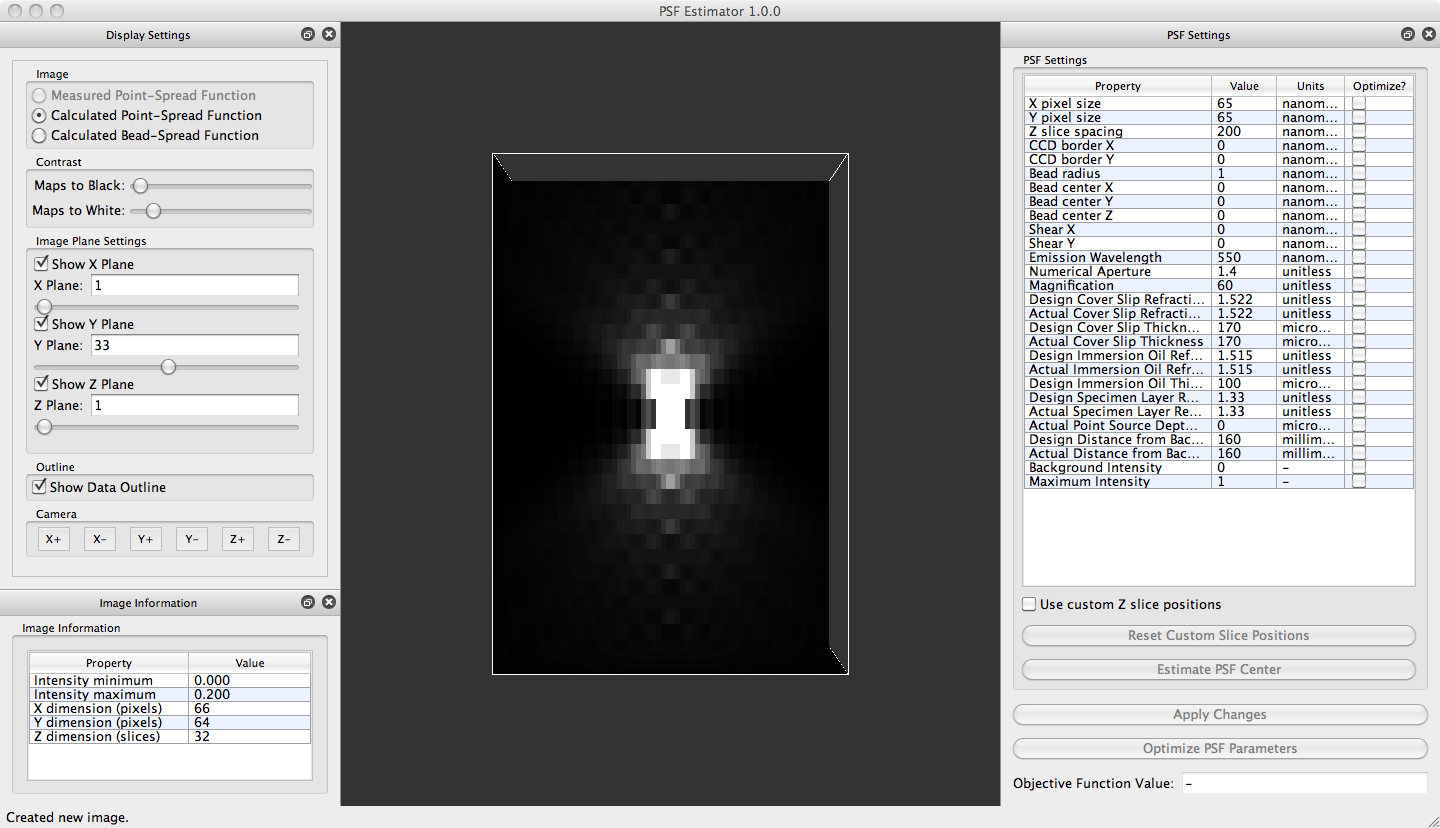
\includegraphics[scale=0.3]{images/ProgramWindow}
  \caption{The PSF Estimator program window.}
  \label{fig:ProgramWindow}
\end{figure}

The main program window is organized into several sections. 

\subsubsection{Visualization Panel}

The visualization panel (center) displays PSFs via three orthogonal cutting planes. A measured PSF imported into the program, a calculated PSF, or a calculated bead-spread function (BSF, the image of a spherical bead convolved with the PSF) can be displayed here. Only one of these images may displayed at one time; switching between them enables visual inspection of the PSF fitting results.

\subsubsection{Display Settings}

The \emph{Display Settings} control which PSF image is displayed in the \emph{Visualization Panel} and how it is displayed.

\begin{description}

  \item[Image] \hfill \\
   
   \begin{figure}[h]
    \centering
    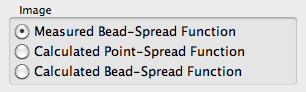
\includegraphics[scale=0.5]{images/ImageControls}
    \caption{Image controls.}
    \label{fig:ImageControls}
  \end{figure}
 
  These controls let you choose which image to display: the measured bead-spread function, the point-spread function corresponding to the current PSF settings, or the bead-spread function corresponding to the current PSF settings.

  \item[Contrast] \hfill \\
  
    \begin{figure}[h]
    \centering
    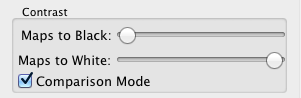
\includegraphics[scale=0.5]{images/ContrastControls}
    \caption{Contrast controls.}
    \label{fig:ContrastControls}
  \end{figure}
  
  Controls which PSF/BSF image voxel value maps to black and which voxel value maps to white.

  \item[Image Plane Settings] \hfill \\
  
    \begin{figure}[h]
    \centering
    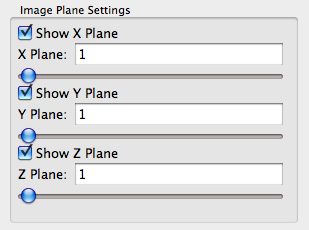
\includegraphics[scale=0.5]{images/ImagePlaneSettingsControls}
    \caption{Image plane settings controls.}
    \label{fig:ImagePlaneSettingsControls}
  \end{figure}
  
  Control which slices through the image in the $yz$, $xz$, and $xy$ planes are displayed and whether those image planes are displayed. The range for the \emph{X Plane} setting is from 1 to the number of voxels into the $x$-direction, and the range for the \emph{Y Plane} and \emph{Z Plane} are similarly defined.

  \item[Outline] \hfill \\
  
  \begin{figure}[h]
    \centering
    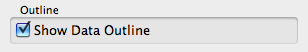
\includegraphics[scale=0.5]{images/OutlineControls}
    \caption{Outline controls.}
    \label{fig:OutlineControls}
  \end{figure}
  
  
  This control enables you to display or hide an outline of the image data.

  \item[Camera] \hfill \\
  
  \begin{figure}[h]
    \centering
    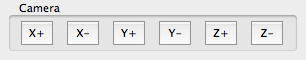
\includegraphics[scale=0.5]{images/CameraControls}
    \caption{Camera controls.}
    \label{fig:CameraControls}
  \end{figure}
  
  These controls consist of six buttons that move the camera to six canonical positions. The +X button moves the camera to look down the positive $x$-axis and the -X button move the camera to look down the negative $x$-axis. The $-Y$, $+Y$, $-Z$, and $+Z$ have similar functions, but operate on different coordinate axes.

\end{description}

\subsubsection{Image Information}

  \begin{figure}[h]
    \centering
    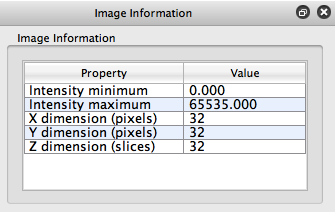
\includegraphics[scale=0.5]{images/ImageInformationControlPanel}
    \caption{Image information control panel.}
    \label{fig:ImageInformationControlPanel}
  \end{figure}


The \emph{Image Information} control panel displays information about the image currently displayed in the \emph{Visualization Panel}. Information includes the minimum and maximum voxel intensity of the image and the size of the image in the $X$-, $Y$-, and $Z$-dimensions.

\subsubsection{PSF Settings}

\begin{figure}[h]
  \centering
  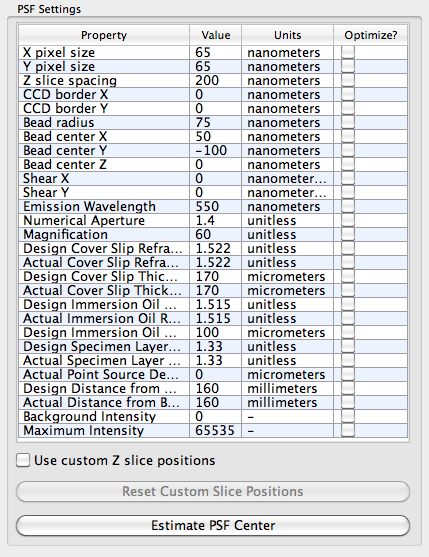
\includegraphics[scale=0.5]{images/PSFSettingsControlPanel}
  \caption{PSF settings control panel.}
  \label{fig:PSFSettingsControlPanel}
\end{figure}

The PSF settings table is used to set parameters for the analytical PSF and BSF models. These parameters are described in Section \ref{sec:PointSpreadFunctionSettings} of this manual.

\subsection{Menu Bar}

The menu bar in PSF Estimator contains three menus that provide various commands. Each menu is described in more detail below.

\subsubsection{File Menu}

The \emph{File Menu} features options for creating PSFs of arbitrary size, opening images, saving PSF images, and loading and saving program sessions.

\begin{description}
  \item[New Image] \hfill \\
  Creates a new PSF with default settings. The size and voxel spacing of the new image can be set prior to the creation of the image. This option is useful for generating a theoretical PSF at arbitrary sampling rates when the PSF parameters are known.

  \item[Open Image...] \hfill \\
  Opens image data. 3D TIFF, VTK, and LSM files are supported. Sequences of 2D TIFF images currently cannot be imported.

  \item[Save PSF Image...] \hfill \\
   Saves the point-spread function image to a file. The image can be exported as a 3D TIFF, VTK, or LSM image.
   
  \item[Save BSF Image...] \hfill \\
  Saves the bead-spread function image to a file. The image can be exported as a 3D TIFF, VTK, or LSM image.
  
  \item[Load Session...] \hfill \\
  Loads the program session file that contains all the program settings from a previous session. This option enables you to do some work in PSF Estimator, save some work, restart the program, and continue where you left off.
  
  \item[Save Session...] \hfill \\
  Save the program session file that contains all the current program settings.
  
  \item[Exit] \hfill \\
  Exits the program. \textbf{Macintosh users:} The \emph{Quit} menu item appears under the \emph{PSFEstimator} menu instead of the \emph{File} menu.

\end{description}
\subsubsection{Edit Menu}

\begin{description}

  \item[Copy] \hfill \\
  Copies text in a text field.
  
  \item[Paste] \hfill \\
  Pastes text into a text field.
  
\end{description}

\subsubsection{Window Menu}

\begin{description}

  \item[About PSFEstimator] \hfill \\
  Shows a window with information about PSF Estimator. \textbf{Macintosh users:} The \emph{About PSFEstimator} menu item appears under the \emph{PSFEstimator} menu instead of the \emph{Window} menu. 

  \item[Display Window] \hfill \\
  Shows/hides the \emph{Display Settings Control Panel}. If you close the \emph{Display Settings Control Panel}, you can show it again with this menu item.
  
  \item[Image Information] \hfill \\
    Shows/hides the \emph{Image Information Control Panel}. If you close the \emph{Image Information Control Panel}, you can show it again with this menu item.
  
  \item[PSF Settings] \hfill \\
  Shows/hides a separate panel that displays the fluorescence images simulated by FluoroSim.

\end{description}

\section{Point-Spread Function Settings}
\label{sec:PointSpreadFunctionSettings}

\subsection{Gibson-Lanni PSF Model for Widefield Microscopes}

\begin{description}

  \item[X pixel size] \hfill \\
   The physical size of the pixel in the $x$ direction.
  
  \item[Y pixel size] \hfill \\
   The physical size of the pixel in the $y$ direction.
  
  \item[Z slice spacing] \hfill \\
   The spacing between slices in the images.
  
  \item[Bead radius] \hfill \\
   The radius of the spherical bead used to generate the measured BSF images.
  
  \item[Bead center X] \hfill \\
   The position of the bead center in the $x$ direction. The origin is defined to be the center of the measured BSF image.
  
  \item[Bead center Y] \hfill \\
   The position of the bead center in the $y$ direction. The origin is defined to be the center of the measured BSF image.
  
  \item[Bead center Z] \hfill \\
   The position of the bead center in the $z$ direction. The origin is defined to be the center of the measured BSF image.
    
  \item[Shear in X] \hfill \\
Models lateral stage movement in the $x$-direction as a linear function directly proportional to the $z$-depth of the focal plane. The $x$-offset in the shear direction is defined as
\begin{equation}
x_{\mathrm{offset}} = m_{x} z
\end{equation}
where $m_{x}$ is the \emph{Shear in X} setting value and $z$ is the focal plane depth. The $x_{\mathrm{offset}}$ is added to the $x$-coordinate of each voxel position during image generation.

  \item[Shear in Y] \hfill \\
   Same as \emph{Shear in X} but in the $y$-direction.

  \item[Emission Wavelength] \hfill \\
   The dominant wavelength in the emission spectrum from the fluorophores in the fluorescently labeled bead.
  
  \item[Numerical Aperture] \hfill \\
   The numerical aperture of the microscope objective lens.
  
  \item[Magnification] \hfill \\
   The magnification of the microscope objective lens.

  \item[Design Cover Slip Refractive Index] \hfill \\
   The cover slip refractive index for which the objective lens was designed.
  
  \item[Actual Cover Slip Refractive Index] \hfill \\
   The actual cover slip refractive index used in the setup for imaging the bead.
  
  \item[Design Cover Slip Thickness] \hfill \\
   The cover slip thickness for which the objective lens was designed.
  
  \item[Actual Cover Slip Thickness] \hfill \\
   The actual cover slip thickness used in the setup for imaging the bead.
  
  \item[Design Immersion Oil Refractive Index] \hfill \\
   The immersion oil refractive index for which the objective lens was designed.
  
  \item[Actual Immersion Oil Refractive Index] \hfill \\
   The actual immersion oil refractive index used in the setup for imaging the bead.
  
  \item[Design Immersion Oil Thickness] \hfill \\
   The immersion oil thickness for which the objective lens was designed.
  
  \item[Design Specimen Layer Refractive Index] \hfill \\
   The specimen layer refractive index for which the objective function was designed. The specimen layer lays below the cover slip.
  
  \item[Actual Specimen Layer Refractive Index] \hfill \\
   The actual specimen layer refractive index in the setup for imaging the bead.
  
  \item[Actual Point Source Depth in Specimen Layer] \hfill \\
   The depth of the specimen below the coverslip.
  
  \item[Design Distance from Back Focal Plane to Detector] \hfill \\
   The design distance from the back focal plane of the objective lens to the CCD camera.
  
  \item[Actual Distance from Back Focal Plane to Detector] \hfill \\
   The actual distance from the back focal plane of the objective lens to the CCD camera.
  
  \item[Background Intensity] \hfill \\
   A uniform background intensity added to each voxel intensity value.
  
  \item[Maximum Intensity] \hfill \\
   The maximum intensity value in calculated PSF or BSF.
      
\end{description}

\subsection{Gaussian PSF Model for Confocal Microscopes}

\section{Version History}

\subsection{Version 1.0.0}

\noindent
Changes from previous release:
\begin{itemize}
\item Initial program release.
\end{itemize}

%\noindent
%Known issues:
%\begin{itemize}

%\item (Bug 11) The saved FluoroSim comparison image is not always loaded when file is re-opened.

%\item (Bug 12) The size of the imported PSF is not reported correctly in the Point-Spread Function Editor.

%\end{itemize}

\end{document}  
